% Ensemble Anomaly Maps - Evaluation Metrics Presentation
% Auto-generated presentation template with evaluation results
% 
% To regenerate figures and metrics, run:
%   python tools/compute_presentation_metrics.py
%
\documentclass[aspectratio=169,11pt]{beamer}

\usetheme{default}
\usecolortheme{whale}

\usepackage{graphicx}
\usepackage{booktabs}
\usepackage{csvsimple}
\usepackage{amsmath}

\title{Ensemble Anomaly Detection}
\subtitle{Evaluation Metrics and Performance Analysis}
\author{Anomaly Detection Pipeline}
\date{\today}

\begin{document}

\begin{frame}
\titlepage
\end{frame}

% =============================================================================
% Evaluation Metrics Overview
% =============================================================================
\begin{frame}{Evaluation Metrics Overview}
\begin{columns}
\begin{column}{0.5\textwidth}
\textbf{Classification Metrics:}
\begin{itemize}
    \item \textbf{AUROC}: Area Under ROC Curve
    \begin{itemize}
        \item Measures discrimination ability
        \item 1.0 = perfect, 0.5 = random
    \end{itemize}
    \item \textbf{AUPRC}: Area Under PR Curve
    \begin{itemize}
        \item Better for imbalanced data
        \item Baseline = class prevalence
    \end{itemize}
\end{itemize}
\end{column}
\begin{column}{0.5\textwidth}
\textbf{Operational Metrics:}
\begin{itemize}
    \item \textbf{Precision@k}: Precision in top k\%
    \begin{itemize}
        \item Useful for anomaly prioritization
    \end{itemize}
    \item \textbf{Recall@FPR}: Recall at fixed FPR
    \begin{itemize}
        \item Controls false alarm rate
    \end{itemize}
\end{itemize}
\end{column}
\end{columns}
\vspace{1em}
\footnotesize{95\% CIs computed via bootstrap (2000 resamples)}
\end{frame}

% =============================================================================
% ROC Curve
% =============================================================================
\begin{frame}{ROC Curve Analysis}
\begin{columns}
\begin{column}{0.6\textwidth}
% NOTE: Run tools/compute_presentation_metrics.py to generate this figure
\IfFileExists{outputs/summary/predictions_roc.png}{%
    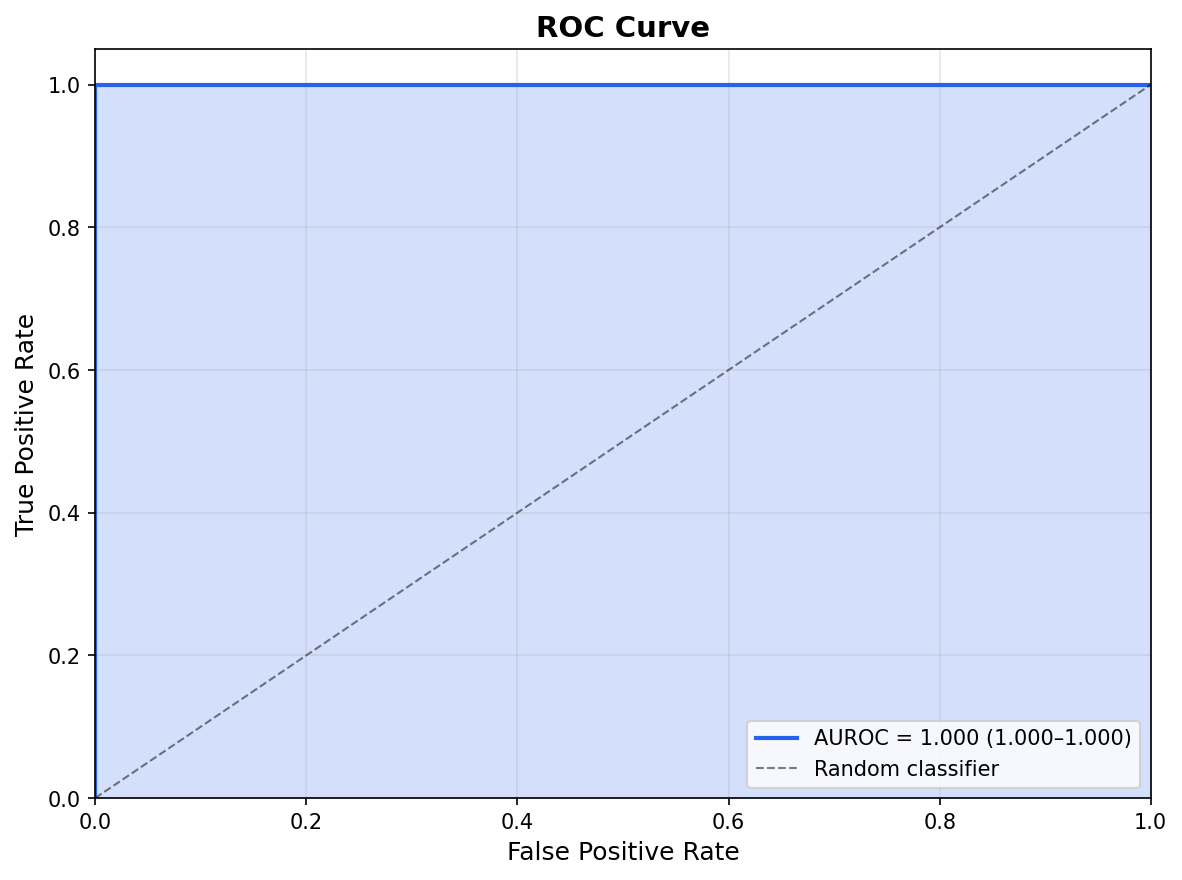
\includegraphics[width=\textwidth]{outputs/summary/predictions_roc.png}
}{%
    \fbox{\parbox{\textwidth}{%
        \centering
        \vspace{3cm}
        \textbf{ROC Curve Placeholder}\\[1em]
        Run the following command to generate:\\[0.5em]
        \texttt{python tools/compute\_presentation\_metrics.py}
        \vspace{3cm}
    }}
}
\end{column}
\begin{column}{0.4\textwidth}
\textbf{Interpretation:}
\begin{itemize}
    \item Upper-left = better performance
    \item Diagonal = random classifier
    \item Area = probability of correct ranking
\end{itemize}
\vspace{1em}
\textbf{Key Points:}
\begin{itemize}
    \item Compare methods visually
    \item Note confidence intervals
    \item Consider operating points
\end{itemize}
\end{column}
\end{columns}
\end{frame}

% =============================================================================
% Precision-Recall Curve
% =============================================================================
\begin{frame}{Precision-Recall Curve Analysis}
\begin{columns}
\begin{column}{0.6\textwidth}
% NOTE: Run tools/compute_presentation_metrics.py to generate this figure
\IfFileExists{outputs/summary/predictions_pr.png}{%
    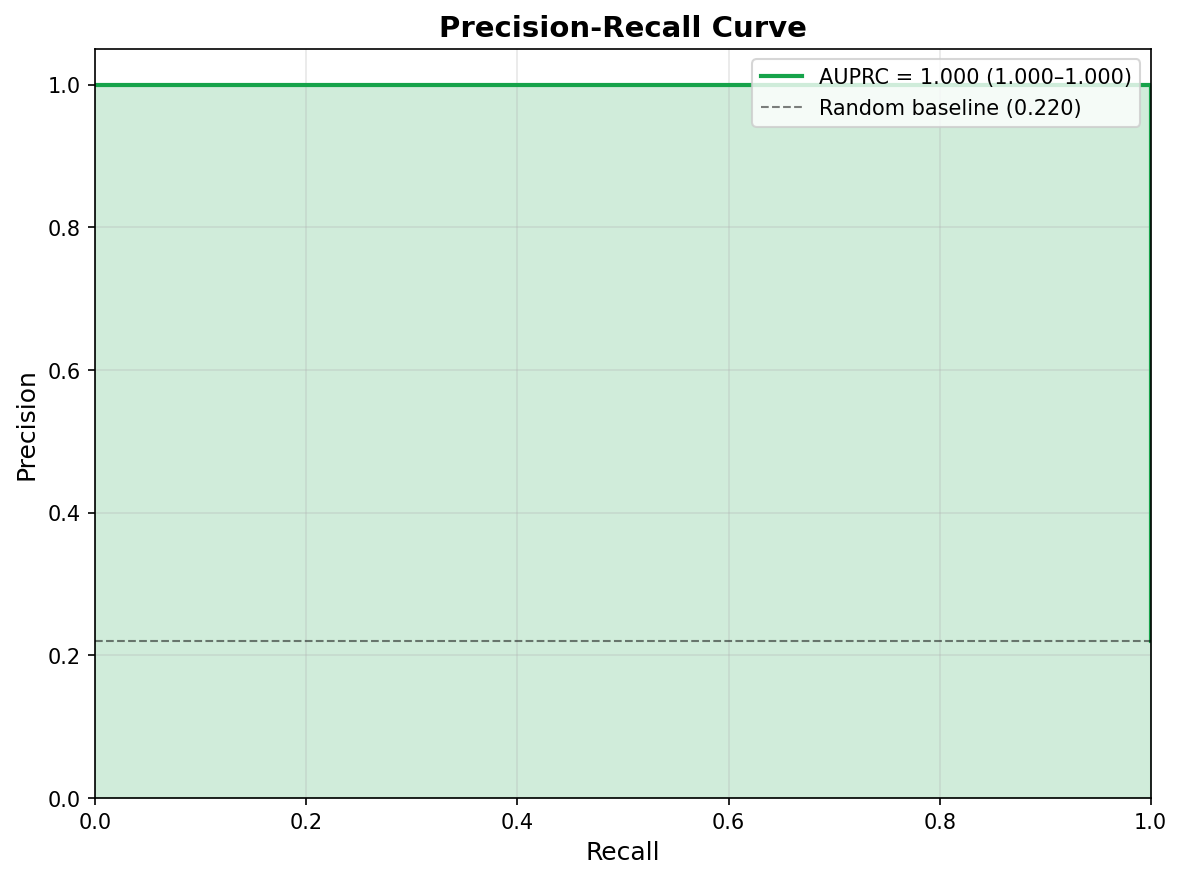
\includegraphics[width=\textwidth]{outputs/summary/predictions_pr.png}
}{%
    \fbox{\parbox{\textwidth}{%
        \centering
        \vspace{3cm}
        \textbf{PR Curve Placeholder}\\[1em]
        Run the following command to generate:\\[0.5em]
        \texttt{python tools/compute\_presentation\_metrics.py}
        \vspace{3cm}
    }}
}
\end{column}
\begin{column}{0.4\textwidth}
\textbf{Interpretation:}
\begin{itemize}
    \item Upper-right = better
    \item Horizontal line = random baseline
    \item More informative for rare events
\end{itemize}
\vspace{1em}
\textbf{Key Points:}
\begin{itemize}
    \item Preferred for imbalanced data
    \item Baseline = class prevalence
    \item Focus on high-recall region
\end{itemize}
\end{column}
\end{columns}
\end{frame}

% =============================================================================
% Score Distributions
% =============================================================================
\begin{frame}{Score Distributions}
\begin{columns}
\begin{column}{0.65\textwidth}
% NOTE: Run tools/compute_presentation_metrics.py to generate this figure
\IfFileExists{outputs/summary/score_distributions.png}{%
    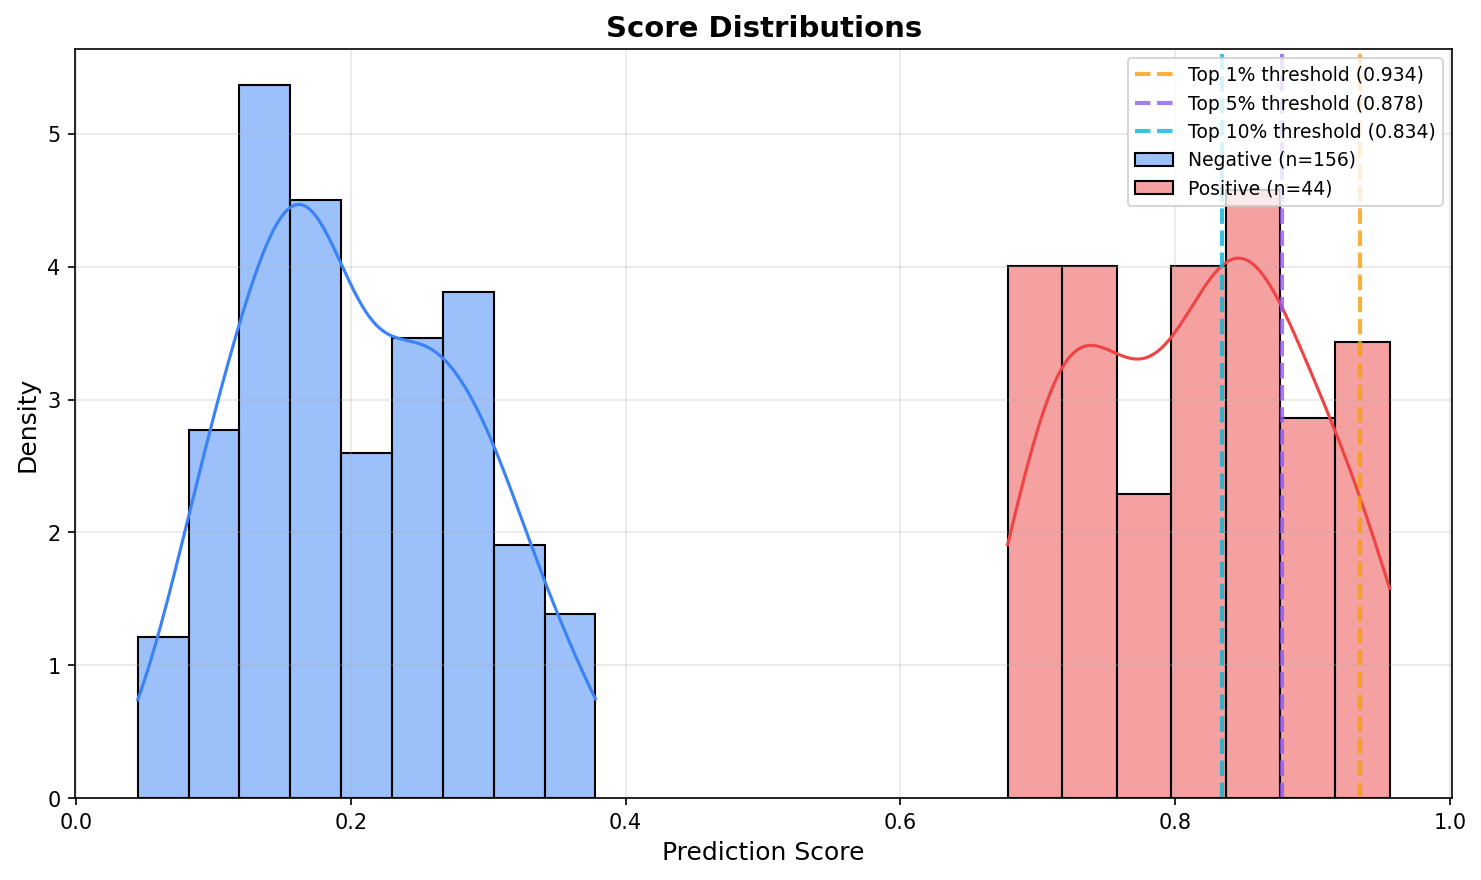
\includegraphics[width=\textwidth]{outputs/summary/score_distributions.png}
}{%
    \fbox{\parbox{\textwidth}{%
        \centering
        \vspace{3cm}
        \textbf{Score Distribution Placeholder}\\[1em]
        Run the following command to generate:\\[0.5em]
        \texttt{python tools/compute\_presentation\_metrics.py}
        \vspace{3cm}
    }}
}
\end{column}
\begin{column}{0.35\textwidth}
\textbf{What to look for:}
\begin{itemize}
    \item Class separation
    \item Score calibration
    \item Threshold selection
\end{itemize}
\vspace{1em}
\textbf{Top-k Thresholds:}
\begin{itemize}
    \item Top 1\% = highest priority
    \item Top 5\% = high priority
    \item Top 10\% = moderate priority
\end{itemize}
\end{column}
\end{columns}
\end{frame}

% =============================================================================
% Metrics Summary Table
% =============================================================================
\begin{frame}{Metrics Summary}
\begin{center}
% NOTE: This table can be auto-populated from outputs/summary/metrics_summary.csv
% For now, we show a template that can be manually updated

\IfFileExists{outputs/summary/metrics_summary.csv}{%
    \begin{tabular}{lcc}
    \toprule
    \textbf{Metric} & \textbf{Value} & \textbf{95\% CI} \\
    \midrule
    AUROC & \textit{See CSV} & \textit{See CSV} \\
    AUPRC & \textit{See CSV} & \textit{See CSV} \\
    \midrule
    Precision@1\% & \textit{See CSV} & -- \\
    Precision@5\% & \textit{See CSV} & -- \\
    Precision@10\% & \textit{See CSV} & -- \\
    \midrule
    Recall@1\%FPR & \textit{See CSV} & -- \\
    Recall@5\%FPR & \textit{See CSV} & -- \\
    \bottomrule
    \end{tabular}
    
    \vspace{1em}
    \footnotesize{Load actual values from: \texttt{outputs/summary/metrics\_summary.csv}}
}{%
    \fbox{\parbox{0.8\textwidth}{%
        \centering
        \vspace{1cm}
        \textbf{Metrics Table Placeholder}\\[1em]
        Run the following command to generate metrics:\\[0.5em]
        \texttt{python tools/compute\_presentation\_metrics.py}\\[1em]
        Results will be saved to: \texttt{outputs/summary/metrics\_summary.csv}
        \vspace{1cm}
    }}
}
\end{center}
\end{frame}

% =============================================================================
% Interpretation Guide for Chemists
% =============================================================================
\begin{frame}{Interpretation Guide for Chemists}
\begin{columns}
\begin{column}{0.5\textwidth}
\textbf{What the metrics mean:}
\begin{itemize}
    \item \textbf{AUROC > 0.8}: Good discrimination
    \item \textbf{AUROC > 0.9}: Excellent discrimination
    \item \textbf{AUPRC}: Compare to baseline (class prevalence)
\end{itemize}
\vspace{1em}
\textbf{Practical recommendations:}
\begin{itemize}
    \item Use Top 1\% for initial screening
    \item Expand to Top 5\% for broader coverage
    \item Consider cost/benefit for threshold
\end{itemize}
\end{column}
\begin{column}{0.5\textwidth}
\textbf{Anomaly prioritization:}
\begin{enumerate}
    \item Sort frames by anomaly score
    \item Inspect top-ranked frames first
    \item Use visualization tools to examine
    \item Document findings for follow-up
\end{enumerate}
\vspace{1em}
\textbf{Confidence intervals:}
\begin{itemize}
    \item Narrow CI = stable estimate
    \item Wide CI = more data needed
    \item Overlapping CIs = no significant difference
\end{itemize}
\end{column}
\end{columns}
\end{frame}

% =============================================================================
% How to Regenerate
% =============================================================================
\begin{frame}[fragile]{How to Regenerate Figures and Metrics}
\textbf{To regenerate all figures and metrics:}

\begin{verbatim}
# Using default settings (auto-detect predictions)
python tools/compute_presentation_metrics.py

# Using specific predictions file
python tools/compute_presentation_metrics.py \
    --predictions outputs/predictions.csv \
    --out-dir outputs/summary \
    --bootstrap 2000 \
    --seed 42

# Dry run (check inputs without generating outputs)
python tools/compute_presentation_metrics.py --dry-run
\end{verbatim}

\vspace{1em}
\textbf{Output files:}
\begin{itemize}
    \item \texttt{outputs/summary/predictions\_roc.png} - ROC curve
    \item \texttt{outputs/summary/predictions\_pr.png} - PR curve
    \item \texttt{outputs/summary/score\_distributions.png} - Score distributions
    \item \texttt{outputs/summary/metrics\_summary.csv} - All metrics
\end{itemize}
\end{frame}

\end{document}
